\chapter{Reaktor Kontinu dan Proses Industri}\label{ch:b2:continuous-reactors}

Di laboratorium, reaksi dijalankan di dalam labu: pereaksi dimasukkan,
campurannya diaduk selama satu jam, reaksinya dihentikan, dan produknya
diisolasi. Pabrik yang membuat produk yang sama dalam ribuan ton bekerja
dengan cara lain. Reaktornya tidak pernah dikosongkan: pereaksi mengalir
masuk di satu ujung, produk mengalir keluar di ujung yang lain, siang dan
malam, dan komposisi di dalamnya tidak berubah terhadap waktu. Dua
pertanyaan lalu menggantikan ``berapa lama?'': seberapa besar reaktor
harus dibuat untuk \omterm{def:b2:continuous-reactors:conversion}{konversi} tertentu, dan bagaimana kalor reaksi dibuang
sebelum memanaskan reaktor sampai tak terkendali? Bab ini menuliskan
neraca massa dan neraca energi untuk dua \omterm{def:b2:continuous-reactors:reactors}{reaktor kontinu} ideal, yaitu
tangki berpengaduk dan pipa, membandingkan keduanya, dan menunjukkan
bagaimana sebuah reaktor dapat mempunyai beberapa keadaan yang mungkin,
salah satunya berupa \omterm{def:b2:continuous-reactors:runaway}{pelarian termal}.

\begin{recall}
Jilid Tahun 1: laju reaksi, hukum laju dan orde, hukum terintegrasi untuk
reaktor tertutup (kini disebut \omterm{def:b2:continuous-reactors:reactors}{reaktor batch}), waktu paruh, hukum
Arrhenius $k = A\,\mathrm e^{-E_a/RT}$, reaksi berurutan.
\Cref{ch:b2:reaction-enthalpy}: kalor yang dilepaskan pada tekanan tetap;
\cref{ch:b2:equilibrium-shifts}: \omterm{def:b2:equilibrium-shifts:single-pass}{konversi sekali lewat}, \omterm{def:b2:equilibrium-shifts:single-pass}{daur ulang}. Dari
fisika: neraca sistem terbuka dalam aliran tunak (yang masuk dikurangi
yang keluar sama dengan yang terakumulasi).
\end{recall}

\begin{omfigure}
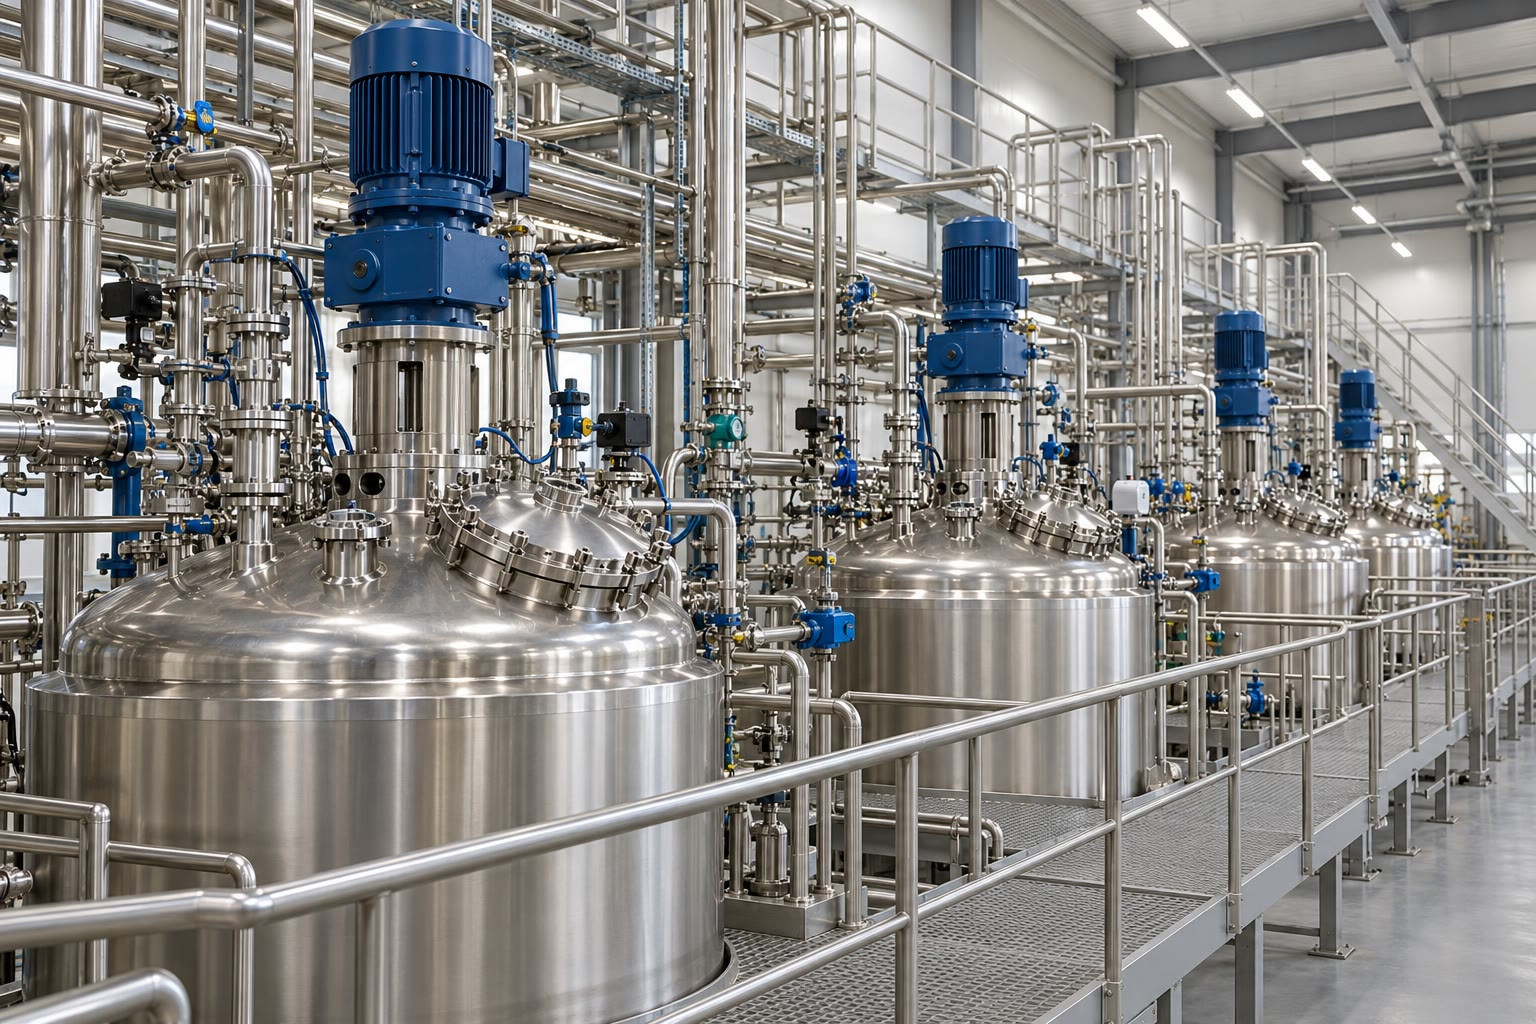
\includegraphics[width=0.6\linewidth]{images/book3/ai/b2-05-stirred-tanks.jpg}

{\small Reaktor tangki berpengaduk di sebuah pabrik kimia: setiap bejana
membawa motor dan kotak roda giginya, dengan poros pengaduk yang turun ke
dalam campuran reaksi; pipa-pipanya membawa umpan dan mengeluarkan produk
serta air pendingin.}
\end{omfigure}

\section{Dari batch ke kontinu}

\begin{definition}[Jenis-jenis reaktor]\label{def:b2:continuous-reactors:reactors}
Yang disebut \emph{reaktor batch}\index{reaktor batch} adalah bejana
tertutup tempat reaksi berlangsung tanpa aliran materi masuk atau keluar.
Yang disebut \emph{reaktor kontinu}\index{reaktor kontinu} adalah reaktor
yang dilewati aliran materi yang tunak. Dua reaktor kontinu ideal dipakai
sebagai model:
\begin{itemize}
  \item \emph{reaktor tangki berpengaduk kontinu}
\index{reaktor tangki berpengaduk kontinu} (CSTR), yang diaduk begitu baik sehingga isinya
        seragam, dan karena itu identik dengan aliran yang keluar darinya;
  \item \emph{reaktor alir sumbat}\index{reaktor alir sumbat} (PFR), sebuah
        pipa yang dilewati fluida tanpa pencampuran di sepanjang aliran,
        dengan setiap irisan fluida maju seperti piston sambil bereaksi.
\end{itemize}
\end{definition}

Sebuah \omterm{def:b2:continuous-reactors:reactors}{reaktor kontinu} dikatakan bekerja dalam \emph{operasi tunak} jika
tidak ada apa pun di dalamnya yang berubah terhadap waktu: aliran, suhu,
dan komposisi di setiap titik tetap. Kita meninjau satu reaksi
$\mathrm A \to$ produk, umpan cair dengan massa jenis tetap (sehingga laju
alir volumetrik $Q_v$ sama di saluran masuk dan saluran keluar), dengan
konsentrasi $c_{A,0}$ di saluran masuk.

\begin{definition}[Waktu tinggal]\label{def:b2:continuous-reactors:residence-time}
Yang disebut \emph{waktu tinggal}\index{waktu tinggal} \omterm{def:b2:continuous-reactors:reactors}{reaktor kontinu}
bervolume $V$ yang diumpani dengan laju alir volumetrik $Q_v$ adalah
$\tau = V/Q_v$: waktu rata-rata yang dihabiskan suatu volume fluida di
dalamnya.
\end{definition}

\begin{definition}[Konversi]\label{def:b2:continuous-reactors:conversion}
Yang disebut \emph{konversi}\index{konversi} pereaksi A adalah
$X = (F_{A,0} -
F_A)/F_{A,0}$, dengan $F_{A,0}$ dan $F_A$ laju alir molar A
yang masuk ke dan keluar dari reaktor; untuk \omterm{def:b2:continuous-reactors:reactors}{reaktor batch},
$X = (n_{A,0} -
n_A)/n_{A,0}$. Pada massa jenis tetap,
$X = 1 - c_A/c_{A,0}$.
\end{definition}

\omterm{def:b2:continuous-reactors:conversion}{Konversi} mengacu pada satu pereaksi, dan pada sebuah reaktor atau satu
kali lewat; rasio kemajuan akhir dalam jilid Tahun 1 mengacu pada sebuah
reaksi dan pereaksi pembatasnya. Untuk satu reaksi yang pereaksi
pembatasnya A, keduanya berimpit.

\begin{proposition}[Reaktor batch]\label{prop:b2:continuous-reactors:batch}
Dalam \omterm{def:b2:continuous-reactors:reactors}{reaktor batch} bervolume tetap, reaksi orde satu mencapai \omterm{def:b2:continuous-reactors:conversion}{konversi}
$X = 1 - \mathrm e^{-kt}$ setelah waktu $t$, dan reaksi orde dua dengan
konsentrasi awal yang sama $c_0$ mencapai \omterm{def:b2:continuous-reactors:conversion}{konversi}
$X =
kc_0t/(1 + kc_0t)$.
\end{proposition}

\begin{proof}
Ini adalah hukum laju terintegrasi dari jilid Tahun 1,
$c_A = c_{A,0}
\mathrm e^{-kt}$ dan $1/c_A = 1/c_{A,0} + kt$, yang
dituliskan dengan $X = 1 -
c_A/c_{A,0}$.
\end{proof}

\section{Reaktor tangki berpengaduk kontinu}

\begin{omfigure}
\begin{tikzpicture}[font=\small, >={Stealth}]
  % batch
  \pic[transform shape] at (0,0) {rbflask={0.6}{omDef!20}};
  \node[below] at (0,-0.15) {batch};
  % CSTR
  \begin{scope}[xshift=4.2cm]
    \draw[thick, fill=omDef!15] (-1.2,0) rectangle (1.2,2.4);
    \draw[thick] (0,3.0) -- (0,0.5);
    \draw[thick, fill=gray!40] (-0.5,0.45) rectangle (0.5,0.6);
    \draw[thick, fill=gray!30] (-0.25,3.0) rectangle (0.25,3.35);
    \draw[->, thick, omDef] (-2.8,2.0) -- (-1.2,2.0) node[pos=0.0, above, anchor=south west, inner sep=1pt] {$Q_v$, $c_{A,0}$};
    \draw[->, thick, omThm] (1.2,0.3) -- (2.5,0.3) node[pos=1, below] {$Q_v$, $c_A$};
    \node[fill=omDef!15, inner sep=1pt] at (0.62,1.5) {$V$, $c_A$};
    \node[below] at (0,-0.15) {tangki berpengaduk};
  \end{scope}
  % PFR
  \begin{scope}[xshift=8.4cm, yshift=1.0cm]
    \draw[thick, fill=omDef!10] (0,0) rectangle (4.2,0.7);
    \fill[omThm!25] (2.0,0) rectangle (2.35,0.7);
    \draw[thick] (2.0,0) -- (2.0,0.7) (2.35,0) -- (2.35,0.7);
    \node[above] at (2.17,0.75) {$\dd V$};
    \draw[->, thick, omDef] (-0.9,0.35) -- (0,0.35) node[pos=0, above] {$F_{A,0}$};
    \draw[->, thick, omThm] (4.2,0.35) -- (5.0,0.35) node[pos=1, above] {$F_A$};
    \node[below] at (1.0,0) {$F_A(V)$};
    \node[below] at (2.1,-1.15) {pipa alir sumbat};
  \end{scope}
\end{tikzpicture}

{\small Tiga reaktor ideal. Labu batch; tangki berpengaduk yang isinya
seragam dan sama dengan aliran keluarannya; pipa yang dilewati aliran
sumbat, tempat laju alir A berkurang dari irisan ke irisan.}
\end{omfigure}

\begin{proposition}[Neraca tangki berpengaduk]\label{prop:b2:continuous-reactors:cstr-balance}
Dalam operasi tunak, tangki berpengaduk bervolume $V$ tempat A hilang
dengan laju $r$ (mol per liter per detik) memenuhi
\[
  F_{A,0} - F_A - rV = 0, \qquad\text{yaitu}\qquad c_{A,0} - c_A = r\,\tau ,
\]
dengan laju yang dievaluasi pada komposisi dan suhu keluaran.
\end{proposition}

\begin{proof}
Neraca A di dalam tangki selama $\dd t$: yang masuk, $F_{A,0}\dd t$,
dikurangi yang keluar, $F_A\dd t$, dikurangi yang bereaksi, $rV\dd t$,
sama dengan akumulasi, yang bernilai nol dalam operasi tunak. Karena
tangki itu seragam, lajunya sama di mana-mana dan sama dengan laju pada
aliran keluaran. Bagilah dengan $Q_v$.
\end{proof}

\begin{theorem}[Konversi dalam tangki berpengaduk]\label{thm:b2:continuous-reactors:cstr}
Untuk reaksi orde satu, $X = \dfrac{k\tau}{1 + k\tau}$; untuk reaksi orde
dua dengan konsentrasi umpan yang sama $c_0$ untuk kedua pereaksi, $X$
adalah akar dalam $[0, 1]$ dari $Da\,(1 - X)^2 = X$, dengan
$Da =
kc_0\tau$.
\end{theorem}

\begin{proof}
Orde 1: $r = kc_A$, sehingga $c_{A,0} - c_A = k\tau c_A$,
$c_A = c_{A,0}/(1 + k\tau)$ dan $X = 1 - 1/(1 + k\tau)$. Orde 2:
$r = kc_A^2$ (kedua konsentrasi tetap sama),
$c_0X = k\tau c_0^2(1 - X)^2$.
\end{proof}

Gugus tak berdimensi $Da = k\tau$ (atau $kc_0\tau$), yaitu bilangan
Damköhler, membandingkan \omterm{def:b2:continuous-reactors:residence-time}{waktu tinggal} dengan skala waktu reaksi:
bilangan ini saja sudah menetapkan \omterm{def:b2:continuous-reactors:conversion}{konversi}.

\begin{method}[Menentukan ukuran reaktor]\label{met:b2:continuous-reactors:size-reactor}
\begin{enumerate}
  \item Tuliskan hukum laju dan \omterm{def:b2:continuous-reactors:conversion}{konversi} $X$ yang dikehendaki.
  \item Dari neraca reaktor yang dipilih, tentukan bilangan Damköhler yang
        memberikan $X$.
  \item Simpulkan $\tau$ dari $Da$ dan tetapan laju pada suhu kerja, lalu
        $V = \tau Q_v$ dari laju alir yang harus diolah.
\end{enumerate}
\end{method}

\section{Reaktor alir sumbat}

\begin{theorem}[Konversi dalam reaktor alir sumbat]\label{thm:b2:continuous-reactors:pfr}
Dalam operasi tunak, laju alir A di sepanjang pipa alir sumbat memenuhi
$\dd F_A/\dd V = -r$. Untuk reaksi orde satu, hal ini memberikan
$X = 1 -
\mathrm e^{-k\tau}$, dan untuk reaksi orde dua dengan umpan yang
sama $X =
Da/(1 + Da)$: hukum-hukum \omterm{def:b2:continuous-reactors:reactors}{reaktor batch}, dengan \omterm{def:b2:continuous-reactors:residence-time}{waktu tinggal}
menggantikan waktu.
\end{theorem}

\begin{proof}
Neraca A pada irisan antara $V$ dan $V + \dd V$: $F_A(V) - F_A(V + \dd V)
- r\,\dd V = 0$, dari situ diperoleh persamaan diferensialnya. Dengan
$F_A = Q_vc_A$ dan $\dd V = Q_v\,\dd t'$ (waktu $t'$ yang telah dihabiskan
sebuah irisan di dalam pipa), persamaan itu menjadi $\dd c_A/\dd t' = -r$:
setiap irisan adalah \omterm{def:b2:continuous-reactors:reactors}{reaktor batch} kecil yang tinggal di dalam pipa
selama $\tau$. Pemisahan variabel untuk $r = kc_A$ memberikan
$c_A = c_{A,0}
\mathrm e^{-k\tau}$ di saluran keluar; untuk $r = kc_A^2$,
$1/c_A - 1/c_0 = k\tau$.
\end{proof}

\begin{omfigure}
\begin{tikzpicture}
\begin{axis}[
  width=0.75\linewidth, height=6cm, xmin=0, xmax=10, ymin=0, ymax=1.05,
  axis x line=bottom, axis y line=left, xlabel={bilangan Damköhler $k\tau$},
  ylabel={konversi $X$}, tick label style={font=\small},
  label style={font=\small}, clip=false,
  legend style={font=\scriptsize, draw=none, at={(0.98,0.05)}, anchor=south east}]
\addplot[omThm, very thick] table[x=Da, y=pfr] {figdata/out/bachelor-2-reactors-a.dat};
\addplot[omProp, thick] table[x=Da, y=five] {figdata/out/bachelor-2-reactors-a.dat};
\addplot[omProp, thick, dashed] table[x=Da, y=two] {figdata/out/bachelor-2-reactors-a.dat};
\addplot[omDef, very thick] table[x=Da, y=cstr] {figdata/out/bachelor-2-reactors-a.dat};
\legend{alir sumbat, 5 tangki seri, 2 tangki seri, 1 tangki}
\draw[dotted] (axis cs:2.303,0) -- (axis cs:2.303,0.9) -- (axis cs:9,0.9);
\fill[omThm] (axis cs:2.303,0.9) circle (1.4pt);
\fill[omDef] (axis cs:9,0.9) circle (1.4pt);
\end{axis}
\end{tikzpicture}

{\small \omterm{def:b2:continuous-reactors:conversion}{Konversi} reaksi orde satu terhadap $k\tau$ dalam reaktor-reaktor
ideal. Untuk \omterm{def:b2:continuous-reactors:conversion}{konversi} 90\,\%, pipa alir sumbat memerlukan
$k\tau = \ln 10 = 2.3$, satu tangki berpengaduk $k\tau = 9$: empat kali
volumenya. Tangki-tangki seri mendekati pipa.}
% (model curves, computed in figdata/bachelor-2/reactors.py)
\end{omfigure}

\begin{proposition}[Tangki atau pipa]\label{prop:b2:continuous-reactors:compare}
Untuk setiap laju yang bertambah seiring konsentrasi A (setiap orde
positif), \omterm{def:b2:continuous-reactors:reactors}{reaktor alir sumbat} mencapai \omterm{def:b2:continuous-reactors:conversion}{konversi} tertentu dengan volume
yang lebih kecil daripada tangki berpengaduk.
\end{proposition}

\begin{proof}
Dari neraca-neracanya, $\tau_{\text{CSTR}} = c_{A,0}X/r(X)$ (laju pada
komposisi keluaran) dan $\tau_{\text{PFR}} = c_{A,0}\int_0^X\dd X'/r(X')$.
Karena $r$ berkurang ketika $X$ bertambah, $1/r(X') \leq 1/r(X)$ pada
$[0, X]$, sehingga integral itu paling besar $X/r(X)$. Secara grafis, pada
diagram $1/r$ terhadap $X$, $\tau$ pipa adalah luas di bawah kurva dan
\omterm{def:b2:continuous-reactors:residence-time}{waktu tinggal} tangki adalah persegi panjang setinggi $1/r(X)$ (gambar di
bawah).
Untuk orde 1: $\ln(1 + k\tau) \leq k\tau$, pernyataan yang sama dalam
bentuk lain.
\end{proof}

Tangki berpengaduk bekerja seluruhnya pada konsentrasi keluaran, yang
terendah dalam sistem itu, sehingga pada laju terendah; pipa memanfaatkan
konsentrasi tinggi di dekat saluran masuknya. Keunggulan tangki terletak
di tempat lain: suhu yang seragam dan mudah dikendalikan, serta
pengoperasian yang sederhana.

\begin{omfigure}
\begin{tikzpicture}
\begin{axis}[
  width=0.62\linewidth, height=5.6cm, xmin=0, xmax=1, ymin=0, ymax=22,
  axis x line=bottom, axis y line=left, xlabel={konversi $X$},
  ylabel={$1/r$ (satuan model)}, tick label style={font=\small},
  label style={font=\small}, clip=false]
\fill[omDef!15] (axis cs:0,0) rectangle (axis cs:0.9,10);
\addplot[omThm, fill=omThm!20, draw=none, domain=0:0.9, samples=60] {1/(1-x)} \closedcycle;
\addplot[black, very thick] table[x=X, y=invr] {figdata/out/bachelor-2-reactors-c.dat};
\draw[omDef, thick] (axis cs:0,10) -- (axis cs:0.9,10) -- (axis cs:0.9,0);
\node[omDef, font=\scriptsize, anchor=south] at (axis cs:0.45,10.2) {tangki berpengaduk: persegi panjang, $\tau = 9$};
\node[omThm, font=\scriptsize, anchor=west] (pf) at (axis cs:0.05,6.5) {alir sumbat: luas berarsir, $\tau = \ln 10$};
\draw[omThm, ->] (axis cs:0.25,6.0) -- (axis cs:0.3,0.8);
\end{axis}
\end{tikzpicture}

{\small Diagram Levenspiel reaksi orde satu ($k = 1$, $c_{A,0} = 1$). Untuk
\omterm{def:b2:continuous-reactors:conversion}{konversi} 90\,\%, tangki berpengaduk memerlukan seluruh persegi panjang,
sedangkan alir sumbat hanya luas berarsir di bawah kurva.}
% (model, computed in figdata/bachelor-2/reactors.py)
\end{omfigure}

\begin{proposition}[Tangki-tangki seri]\label{prop:b2:continuous-reactors:cascade}
$N$ tangki berpengaduk yang sama yang dipasang seri, dengan \omterm{def:b2:continuous-reactors:residence-time}{waktu tinggal}
total $\tau$, mengonversi reaksi orde satu sampai
$X_N = 1 - (1 + k\tau/N)^{-N}$, yang bertambah seiring $N$ dan menuju
nilai alir sumbat $1 - \mathrm e^{-k\tau}$.
\end{proposition}

\begin{proof}
Setiap tangki membagi konsentrasi dengan $1 + k\tau/N$. Lalu
$(1 +
k\tau/N)^{-N} = \exp[-N\ln(1 + k\tau/N)] \to \mathrm e^{-k\tau}$,
karena $N\ln(1 + u/N) \to u$.
\end{proof}

\begin{definition}[Selektivitas]\label{def:b2:continuous-reactors:selectivity}
Jika sebuah pereaksi dapat menghasilkan beberapa produk, yang disebut
\emph{selektivitas}\index{selektivitas} untuk produk yang dikehendaki B
adalah jumlah B yang terbentuk dibagi jumlah pereaksi yang terkonsumsi
(dikalikan rasio stoikiometrinya): besaran ini menyatakan seberapa banyak
dari yang bereaksi berjalan ke arah yang benar.
\end{definition}

\begin{proposition}[Zat antara dalam tangki dan dalam pipa]\label{prop:b2:continuous-reactors:consecutive}
Untuk reaksi berurutan orde satu $\mathrm A \xrightarrow{k_1} \mathrm B
\xrightarrow{k_2} \mathrm C$, dengan umpan berupa A saja, konsentrasi B di
saluran keluar paling besar untuk $\tau = \ln(k_2/k_1)/(k_2 - k_1)$ dalam
\omterm{def:b2:continuous-reactors:reactors}{reaktor alir sumbat} dan untuk $\tau = 1/\sqrt{k_1k_2}$ dalam tangki
berpengaduk; maksimumnya lebih tinggi di dalam pipa.
\end{proposition}

\begin{proof}
Pipa: hukum batch dari jilid Tahun 1, $c_B = c_{A,0}\frac{k_1}{k_2 - k_1}
(\mathrm e^{-k_1\tau} - \mathrm e^{-k_2\tau})$, maksimum ketika turunannya
nol, $k_1\mathrm e^{-k_1\tau} = k_2\mathrm e^{-k_2\tau}$. Tangki:
$c_A =
c_{A,0}/(1 + k_1\tau)$ dan neraca B, $c_B = k_1\tau c_A - k_2\tau c_B$,
memberikan $c_B = c_{A,0}k_1\tau/[(1 + k_1\tau)(1 + k_2\tau)]$, yang
turunannya nol jika $k_1k_2\tau^2 = 1$. Perbandingan kedua maksimum itu
adalah \cref{exo:b2:continuous-reactors:10}.
\end{proof}

\section{Neraca kalor dan keselamatan}

\begin{definition}[Kenaikan suhu adiabatik]\label{def:b2:continuous-reactors:adiabatic-rise}
Yang disebut \emph{kenaikan suhu adiabatik}\index{kenaikan suhu adiabatik}
$\Delta T_{\text{ad}}$ sebuah campuran reaksi adalah kenaikan suhu yang
akan dialaminya jika reaksi berlangsung tuntas dan tidak ada kalor yang
dibuang.
\end{definition}

\begin{proposition}[Kenaikan adiabatik campuran cair]\label{prop:b2:continuous-reactors:adiabatic}
Untuk campuran dengan massa jenis $\rho$ dan kapasitas kalor spesifik
$c_p$, tempat pereaksi A, pada konsentrasi $c_{A,0}$, bereaksi dengan
entalpi $\Delta_r H$ per mol A, kenaikan suhu pada \omterm{def:b2:continuous-reactors:conversion}{konversi} $X$ tanpa
kehilangan kalor adalah
\[
  \Delta T = \frac{(-\Delta_r H)\,c_{A,0}\,X}{\rho\,c_p}, \qquad
  \Delta T_{\text{ad}} = \frac{(-\Delta_r H)\,c_{A,0}}{\rho\,c_p} .
\]
\end{proposition}

\begin{proof}
Untuk satu satuan volume, kalor yang dilepaskan, $(-\Delta_r H)c_{A,0}X$,
memanaskan massa $\rho$ dengan kapasitas kalor $c_p$ (hukum pertama pada
tekanan tetap, dua tahap pada \cref{prop:b2:reaction-enthalpy:flame}).
\end{proof}

Campuran encer aman: kenaikannya hanya beberapa derajat. Campuran pekat
yang sangat \omterm{def:b2:reaction-enthalpy:exothermic}{eksoterm} dapat memanaskan dirinya sendiri sampai ratusan
kelvin, cukup untuk mendidihkan pelarut atau memicu reaksi lain. Selain
itu, laju bertambah secara eksponensial terhadap suhu: kalor mempercepat
reaksi, yang lalu melepaskan kalor lebih cepat lagi.

\begin{proposition}[Keadaan tunak tangki berpengaduk yang didinginkan]\label{prop:b2:continuous-reactors:steady-states}
Untuk tangki berpengaduk dengan umpan pada $T_0$, yang didinginkan oleh
mantel pada $T_0$ dengan koefisien perpindahan kalor dikali luas $UA$,
suhu-suhu tunak $T$ yang mungkin adalah penyelesaian dari
\[
  \underbrace{\Delta T_{\text{ad}}\,X(T)}_{\text{kalor dihasilkan}} =
  \underbrace{(1 + \kappa)(T - T_0)}_{\text{kalor dibuang}}, \qquad
  \kappa = \frac{UA}{Q_v\rho c_p},
\]
dengan $X(T) = k(T)\tau/(1 + k(T)\tau)$ untuk reaksi orde satu. Kalor yang
dihasilkan merupakan kurva berbentuk S terhadap $T$, sedangkan kalor yang
dibuang merupakan garis lurus: perpotongannya dapat berjumlah satu atau
tiga.
\end{proposition}

\begin{proof}
Neraca energi tangki dalam operasi tunak, per satuan waktu: kalor yang
dilepaskan oleh reaksi, $(-\Delta_r H)F_{A,0}X$, keluar bersama aliran
keluaran, yang dipanaskan dari $T_0$ ke $T$, $Q_v\rho c_p(T - T_0)$, dan
melalui mantel, $UA(T - T_0)$. Bagilah dengan $Q_v\rho c_p$. Dengan hukum
Arrhenius, $X(T)$ naik dari 0 ke 1 dalam rentang suhu yang sempit: sebuah
S.
\end{proof}

\begin{omfigure}
\begin{tikzpicture}
\begin{axis}[
  width=0.75\linewidth, height=6.2cm, xmin=300, xmax=470, ymin=0, ymax=250,
  axis x line=bottom, axis y line=left, xlabel={suhu tangki $T$ (K)},
  ylabel={kalor per satuan aliran (K)}, tick label style={font=\small},
  label style={font=\small}, clip=true]
\addplot[omThm, very thick] table[x=T, y=gen] {figdata/out/bachelor-2-reactors-b.dat};
\addplot[omDef, very thick] table[x=T, y=rem] {figdata/out/bachelor-2-reactors-b.dat};
\fill[black] (axis cs:300.03,0.04) circle (2pt);
\fill[white, draw=black] (axis cs:390.4,135.6) circle (2pt);
\fill[black] (axis cs:429.6,194.4) circle (2pt);
\node[font=\scriptsize, anchor=north west, fill=white, inner sep=1pt] at (axis cs:318,58) {dingin, stabil}; \draw[black!60] (axis cs:301.5,2) -- (axis cs:318,52);
\node[font=\scriptsize, anchor=north west] at (axis cs:393,132) {tidak stabil};
\node[font=\scriptsize, anchor=south east] at (axis cs:426,197) {panas, stabil};
\node[omThm, font=\scriptsize, anchor=north west] at (axis cs:440,196) {dihasilkan};
\node[omDef, font=\scriptsize, anchor=south east] at (axis cs:452,232) {dibuang};
\end{axis}
\end{tikzpicture}

{\small Diagram Semenov tangki berpengaduk yang didinginkan (parameter
model). Kalor yang dihasilkan (merah) dan kalor yang dibuang (garis biru)
berpotongan tiga kali. Keadaan tengah tidak stabil: sedikit lebih hangat,
pembangkitan kalor menang dan tangki ``lari'' ke keadaan panas; sedikit
lebih dingin, tangki jatuh kembali ke keadaan dingin.}
% (model, computed in figdata/bachelor-2/reactors.py)
\end{omfigure}

Kestabilan setiap keadaan ditentukan oleh kemiringannya: pada titik
potong tempat garis pembuangan lebih curam daripada kurva pembangkitan,
kenaikan suhu yang kecil membuang lebih banyak kalor daripada yang
dihasilkannya, dan tangki mendingin kembali; tempat kurva pembangkitan
lebih curam, kenaikan kecil memperkuat dirinya sendiri. (Analisis yang
ketat melinearkan neraca yang bergantung pada waktu; di sini analisis itu
diterima tanpa bukti.)

\begin{definition}[Pelarian termal]\label{def:b2:continuous-reactors:runaway}
Yang disebut \emph{pelarian termal}\index{pelarian termal} adalah kenaikan
suhu yang mempercepat dirinya sendiri pada campuran yang bereaksi, yang
pembangkitan kalornya, yang tumbuh secara eksponensial terhadap suhu,
melampaui pembuangan kalornya.
\end{definition}

\begin{method}[Neraca kalor sebuah reaktor]\label{met:b2:continuous-reactors:heat-balance}
\begin{enumerate}
  \item Hitunglah \omterm{def:b2:continuous-reactors:adiabatic-rise}{kenaikan suhu adiabatik}: jika hanya beberapa kelvin,
        reaktor itu aman secara termal.
  \item Jika tidak, hitunglah beban pendinginan, $(-\Delta_r H)F_{A,0}X$
        dikurangi kalor yang dibawa oleh aliran keluaran, lalu periksalah
        bahwa mantel atau koil mampu membuangnya.
  \item Periksalah kestabilan titik operasi (kemiringan pada diagram
        Semenov), serta apa yang akan terjadi jika pendinginan gagal: suhu
        maksimum yang dicapai, $T + \Delta T_{\text{ad}}(1 - X)$ untuk
        pereaksi yang masih ada.
\end{enumerate}
\end{method}

\section{Dari protokol ke pabrik}

Sintesis yang berhasil di dalam labu \qty{1}{L} tidak dapat begitu saja
diperbesar seribu kali. Volume, dan kalor yang dilepaskan, bertambah
sebanding dengan pangkat tiga ukuran; dinding, tempat kalor keluar,
sebanding dengan pangkat duanya. Bejana yang sepuluh kali lebih lebar
mempunyai volume seribu kali lipat tetapi luas pendinginan hanya seratus
kali lipat: reaksi yang tetap suam-suam kuku di dalam labu dapat
mengalami \omterm{def:b2:continuous-reactors:runaway}{pelarian termal} di dalam tangki. Karena itu praktik industri
menambahkan pereaksi yang paling reaktif secara perlahan (reaksi tidak
dapat melepaskan kalor lebih banyak daripada pereaksi yang diumpankan),
mengencerkan, mendinginkan dengan koil internal, atau beralih ke \omterm{def:b2:continuous-reactors:reactors}{reaktor
kontinu} bervolume kecil, yang isinya yang sedikit membatasi apa yang
dapat salah.

\omterm{def:b2:continuous-reactors:selectivity}{Selektivitas} adalah perhatian yang lain. Pabrik tidak membuang apa yang
tidak bereaksi: pabrik memisahkan produk dan mendaur ulang pereaksi,
seperti pada sirkuit amonia. Karena itu pabrik dapat menerima \omterm{def:b2:equilibrium-shifts:single-pass}{konversi
sekali lewat} yang sedang saja jika \omterm{def:b2:continuous-reactors:selectivity}{selektivitasnya} tinggi, sebab setiap
produk samping berarti bahan baku yang hilang dan limbah yang harus
diolah.

\begin{inthelab}[Tangki berpengaduk di meja laboratorium]
Kinetika reaksi yang ditujukan untuk pabrik kontinu diukur dalam reaktor
berpengaduk kecil yang diumpani oleh dua pompa terkalibrasi, dengan sel
konduktivitas atau spektrometer daring di saluran keluar. Mengubah laju
alir berarti mengubah $\tau$; konsentrasi keluaran yang tunak pada setiap
$\tau$ memberikan laju secara langsung, melalui neraca
$r = (c_{A,0} - c_A)/\tau$, tanpa integrasi sama sekali.
\end{inthelab}

\section{Latihan}

\begin{exercise}[$\star$]\label{exo:b2:continuous-reactors:1}
Sebuah tangki berpengaduk \qty{2.0}{m^3} diumpani dengan laju
\qty{0.50}{L/s}. Hitunglah \omterm{def:b2:continuous-reactors:residence-time}{waktu tinggalnya} dalam detik dan dalam jam.
\end{exercise}

\begin{exercise}[$\star$]\label{exo:b2:continuous-reactors:2}
Sebuah reaksi orde satu mempunyai $k = \qty{1.2e-3}{s^{-1}}$ pada suhu
kerja. Hitunglah \omterm{def:b2:continuous-reactors:conversion}{konversi} dalam tangki berpengaduk dan dalam pipa alir
sumbat dengan \omterm{def:b2:continuous-reactors:residence-time}{waktu tinggal} yang sama, \qty{30}{min}.
\end{exercise}

\begin{exercise}[$\star$]\label{exo:b2:continuous-reactors:3}
\omterm{def:b2:continuous-reactors:residence-time}{Waktu tinggal} alir sumbat berapakah yang memberikan \omterm{def:b2:continuous-reactors:conversion}{konversi} 99\,\% untuk
reaksi orde satu dengan $k = \qty{0.020}{s^{-1}}$? Dan untuk tangki
berpengaduk?
\end{exercise}

\begin{exercise}[$\star$]\label{exo:b2:continuous-reactors:4}
Larutan berair \qty{0.50}{mol/L} sebuah pereaksi yang reaksinya
melepaskan \qty{-120}{kJ/mol} ($\rho = \qty{1.0}{kg/L}$, $c_p =
\qty{4.2}{J/(g.K)}$) bereaksi seluruhnya. Hitunglah \omterm{def:b2:continuous-reactors:adiabatic-rise}{kenaikan suhu
adiabatiknya}. Apakah kegagalan pendinginan berbahaya?
\end{exercise}

\begin{exercise}[$\star\star$]\label{exo:b2:continuous-reactors:5}
Untuk reaksi orde dua dengan umpan yang sama ($kc_0 = \qty{0.010}{s^{-1}}$),
hitunglah \omterm{def:b2:continuous-reactors:residence-time}{waktu tinggal} untuk \omterm{def:b2:continuous-reactors:conversion}{konversi} 80\,\% dalam tangki berpengaduk dan
dalam pipa alir sumbat. Bandingkan rasionya dengan rasio untuk reaksi orde
satu.
\end{exercise}

\begin{exercise}[$\star\star$]\label{exo:b2:continuous-reactors:6}
Tiga tangki berpengaduk yang sama dipasang seri, dengan \omterm{def:b2:continuous-reactors:residence-time}{waktu tinggal}
total \qty{10}{min}, mengolah reaksi orde satu dengan
$k = \qty{0.50}{min^{-1}}$. Hitunglah \omterm{def:b2:continuous-reactors:conversion}{konversinya}, lalu bandingkan dengan
satu tangki dan dengan pipa yang \omterm{def:b2:continuous-reactors:residence-time}{waktu tinggal} totalnya sama.
\end{exercise}

\begin{exercise}[$\star\star$]\label{exo:b2:continuous-reactors:7}
Sebuah tangki berpengaduk mengonversi 70\,\% suatu pereaksi (orde satu).
Laju alirnya digandakan. Berapa \omterm{def:b2:continuous-reactors:conversion}{konversi} yang baru? Dengan faktor berapa
volumenya harus diperbesar agar kembali mencapai 70\,\%?
\end{exercise}

\begin{exercise}[$\star\star$]\label{exo:b2:continuous-reactors:8}
Sebuah tangki \qty{5.0}{m^3} bekerja pada \qty{350}{K} dengan umpan
\qty{2.0}{mol/L} pereaksi pada \qty{1.0}{L/s}, yang terkonversi 90\,\%,
$\Delta_r H
= \qty{-80}{kJ/mol}$, $\rho c_p = \qty{4.0}{kJ/(L.K)}$, umpan
pada \qty{330}{K}. Hitunglah kalor yang dilepaskan per detik, kalor yang
dibawa pergi oleh aliran keluaran, dan beban pendinginan mantel.
\end{exercise}

\begin{exercise}[$\star\star$]\label{exo:b2:continuous-reactors:9}
Sebuah labu \qty{1.0}{L} dan sebuah reaktor \qty{1.0}{m^3} mempunyai bentuk
yang sama. Dengan faktor berapa volume, luas dinding, dan rasio keduanya
dikalikan? Jelaskan mengapa reaksi yang mudah didinginkan di dalam labu
dapat mengalami \omterm{def:b2:continuous-reactors:runaway}{pelarian termal} di dalam reaktor.
\end{exercise}

\begin{exercise}[$\star\star\star$]\label{exo:b2:continuous-reactors:10}
Untuk $\mathrm A \to \mathrm B \to \mathrm C$ dengan $k_1 = \qty{0.10}{min^{-1}}$
dan $k_2 = \qty{0.050}{min^{-1}}$, hitunglah \omterm{def:b2:continuous-reactors:residence-time}{waktu tinggal} optimum dan
rendemen maksimum B dalam \omterm{def:b2:continuous-reactors:reactors}{reaktor alir sumbat} dan dalam tangki
berpengaduk, lalu jelaskan mengapa pipa lebih unggul untuk zat antara.
\end{exercise}

\begin{exercise}[$\star\star\star$]\label{exo:b2:continuous-reactors:11}
Dengan diagram Semenov dalam bab ini, uraikan apa yang terjadi jika suhu
pendingin dinaikkan perlahan-lahan, lalu diturunkan lagi perlahan-lahan:
tunjukkan bahwa tangki melompat dari cabang dingin ke cabang panas pada
satu suhu dan kembali pada suhu yang lain (histeresis).
\end{exercise}

\begin{exercise}[$\star\star\star$]\label{exo:b2:continuous-reactors:12}
Sebuah \omterm{def:b2:continuous-reactors:reactors}{reaktor batch} diisi pereaksi \qty{2.0}{mol/L} ($\Delta_r H =
\qty{-100}{kJ/mol}$, $\rho c_p = \qty{4.0}{kJ/(L.K)}$) dan dipanaskan sampai
suhu kerja. Kemudian pendinginan gagal pada \omterm{def:b2:continuous-reactors:conversion}{konversi} 25\,\%. Hitunglah
suhu yang dapat dicapai campuran itu. Dalam operasi semi-batch, pereaksi
yang sama ditambahkan perlahan-lahan dan langsung terkonsumsi begitu
datang, sehingga paling banyak 5\,\% muatan berada dalam keadaan belum
bereaksi: berapa kenaikan suhu terburuk sekarang?
\end{exercise}

\section{Soal: Sabun di dalam Tangki}

\begin{problem}[{Soal akhir pekan --- saponifikasi sebuah ester di dalam
tangki berpengaduk: kinetika, penentuan ukuran untuk konversi 90\,\%,
alternatif berupa pipa dan kaskade, serta neraca kalor}]
\label{pb:b2:continuous-reactors:1}
Etil etanoat disaponifikasi oleh natrium hidroksida,
\ce{CH3COOC2H5 + OH- -> CH3COO- + C2H5OH}, sebuah reaksi orde dua (orde
satu terhadap setiap pereaksi). Sebuah pabrik mengolah \qty{0.50}{L/s}
campuran yang konsentrasi ester dan hidroksidanya di saluran masuk
sama-sama $c_0 =
\qty{0.10}{mol/L}$. Untuk soal ini, ambillah
$k = \qty{0.11}{L/(mol.s)}$ pada suhu kerja dan
$\Delta_r H = \qty{-55}{kJ/mol}$ (nilai yang ditetapkan untuk latihan);
campuran itu mempunyai massa jenis dan kapasitas kalor air,
$\rho = \qty{997}{kg/m^3}$, $c_p = \qty{4.18}{kJ/(kg.K)}$.

\medskip
\noindent\textbf{Bagian I --- Kinetika.}
\begin{enumerate}
  \item Tuliskan hukum lajunya. Mengapa kedua konsentrasi tetap sama?
  \item Dalam labu batch, berapa lama waktu yang diperlukan untuk \omterm{def:b2:continuous-reactors:conversion}{konversi}
        90\,\%?
  \item Hitunglah waktu paruh di dalam labu. Mengapa waktu paruh itu
        bergantung pada $c_0$?
  \item Tuliskan bilangan Damköhler reaksi itu untuk \omterm{def:b2:continuous-reactors:residence-time}{waktu tinggal} $\tau$.
\end{enumerate}

\medskip
\noindent\textbf{Bagian II --- Satu tangki berpengaduk.}
\begin{enumerate}[resume]
  \item Tuliskan neraca ester di dalam tangki dalam operasi tunak.
  \item Tunjukkan bahwa $Da\,(1 - X)^2 = X$.
  \item Hitunglah bilangan Damköhler yang diperlukan untuk $X = 0.90$.
  \item Hitunglah \omterm{def:b2:continuous-reactors:residence-time}{waktu tinggalnya}.
  \item Hitunglah volume tangki.
  \item Konsentrasi manakah yang ``dilihat'' reaksi di mana-mana di dalam
        tangki, dan mengapa tangki itu begitu besar?
\end{enumerate}

\medskip
\noindent\textbf{Bagian III --- Sebuah pipa, sebuah kaskade.}
\begin{enumerate}[resume]
  \item Hitunglah bilangan Damköhler dan volume pipa alir sumbat untuk
        tugas yang sama.
  \item Hitunglah rasio kedua volume itu.
  \item Tiga tangki yang sama dipasang seri: tuliskan hubungan antara
        konsentrasi keluaran dua tangki yang berurutan.
  \item Volume total ketiga tangki yang memberikan 90\,\% adalah
        \qty{0.85}{m^3}. Periksalah hal itu dengan menghitung konsentrasi
        yang keluar dari setiap tangki.
  \item Susunan manakah yang sebaiknya dibangun, dan mengapa satu tangki
        mungkin tetap lebih disukai?
\end{enumerate}

\medskip
\noindent\textbf{Bagian IV --- Kalor.}
\begin{enumerate}[resume]
  \item Hitunglah \omterm{def:b2:continuous-reactors:adiabatic-rise}{kenaikan suhu adiabatik} campuran itu.
  \item Hitunglah kalor yang dilepaskan per detik di dalam tangki.
  \item Apakah pendinginan diperlukan? Apakah \omterm{def:b2:continuous-reactors:runaway}{pelarian termal} mungkin
        terjadi?
  \item Apa yang akan berubah untuk campuran yang diumpankan pada
        \qty{2.0}{mol/L}?
  \item Hitunglah massa natrium etanoat yang dihasilkan per hari.
  \item Jika reaksi dijalankan pada suhu yang lebih tinggi, bagaimana
        volume tangki berubah, dan apa harganya?
  \item Nyatakan volume satu tangki berpengaduk yang mengonversi 90\,\%
        ester pada umpan ini.
\end{enumerate}
\end{problem}
